\clearpage
\section{Quantum Noise}

\begin{tcolorbox}	
\begin{tabular}{p{2.75cm} p{0.2cm} p{10.5cm}}
\textbf{Contributors}  
                       &:& Diamantino Silva, (2017-01-23 - ...)\\
                       &:& Armando Pinto (2017-01-23 - ...)\\
\textbf{Goal}          &:& Simulation and measurement of quantum noise in double homodyne detection.\\
\end{tabular}
\end{tcolorbox}
%
\vspace{2em}
%
%
Quantum noise is an intrinsic property of light, a manifestation of the vaccum field fluctuations
\cite{fox2006}.
%\footnote{Mark Fox, p.132}
Contrarily to the majority of noise sources, that are overcomed by better equipment, quantum noise has a lower bound, given by the Heisenberg uncertanty principle, which cannot be broken. This propertie can be useful in some areas, such in quantum cryptography, were many protocols depend on it to ensure their security.\\
The objective of this work is to develop a numerical model for the quantum noise in a double homodyne detection and to validate the numerical model with experimental results.\\
%
%
\subsection{Theoretical Analysis}
%
\subsubsection{Classical Description}



\subsubsection{Quantum Description}

We start by defining number states $\ket{n}$ (or Fock states), which correspond to states with perfectly fixed number of photons
%\footnote{Loundon, p.184}
\cite{loudon2000}.
Associated to those states are two operators, the creation $\hat{a}^\dagger$ and annihilation $\hat{a}$ operators, which in a simple way, remove or add one photon from a given number state
%\footnote{Mark Fox, p.155}
\cite{fox2006}.
Their action is defined as
%
\begin{center}
	\hspace{-4mm}
	\begin{minipage}{44mm}
		\noindent
		\begin{equation}
			\hat{a} \ket{n} = \sqrt{n} \ket{n-1}
		\end{equation}
	\end{minipage}
	$,\quad$
	\begin{minipage}{52mm}
		\noindent
		\begin{equation}
			\hat{a}^\dagger \ket{n} = \sqrt{n+1} \ket{n+1}
		\end{equation}
	\end{minipage}
	$,\quad$
	\begin{minipage}{35mm}
		\noindent
		\begin{equation}
			\hat{n} \ket{n} = n \ket{n}
		\end{equation}
	\end{minipage}
\end{center}
%
in which $\hat{n} = \hat{a}^\dagger\hat{a}$ is the number operator. Therefore, number states are eigenvectors of the number operator.\\
\\
Coherent states have properties that closely resemble classical electromagnetic waves, and are generated by single-mode lasers well above the threshold.
\cite{loudon2000}
%\footnote{Loudon, p.190}
We can defined them, using number states in the following manner
\begin{equation}
\ket{\alpha} = e^{-\frac{|\alpha|^2}{2}} \sum_{n=0}^\infty \frac{\alpha^n}{\sqrt{n!}} \ket{n}
\end{equation}
in which the complex number $\alpha$ is the sole parameter that characterizes it.
%\footnote{Loudon, p.184}
%\footnote{Loudon, p.186}
In fact, if we calculate the expected number of photons with $\bra{\alpha} \hat{n} \ket{\alpha}$ we will obtain $|\alpha|^2$. The coherent state is an eigenstate of the annihilation operator, $\hat{a}\ket{\alpha} = \alpha \ket{\alpha}$.\\
\\
%
%
Using the creation and annihilation operators, we can define two quadrature operators
\cite{loudon2000}
%\footnote{Loudon, p.138, (4.3.36)}
%
\begin{center}
	\begin{minipage}{41mm}
		\noindent
		\begin{equation}
			\hat{X} = \frac{1}{2} \left( \hat{a}^\dagger + \hat{a} \right)
		\end{equation}
	\end{minipage}
	$,\quad$
	\begin{minipage}{40mm}
		\noindent
		\begin{equation}
			\hat{Y} = \frac{i}{2} \left( \hat{a}^\dagger - \hat{a} \right)
		\end{equation}
	\end{minipage}
\end{center}
%
The expected value of these two operators, using a coherent state $\ket{\alpha}$ are
%
\begin{center}
	\begin{minipage}{37mm}
		\noindent
		\begin{equation}
			\braket{\hat{X}} = \textrm{Re}(\alpha)
		\end{equation}
	\end{minipage}
	$,\quad$
	\begin{minipage}{37mm}
		\noindent
		\begin{equation}
			\braket{\hat{Y}} = \textrm{Im}(\alpha)
		\end{equation}
	\end{minipage}
\end{center}
%
We see that the expected value of these operators give us the real and imaginary part of $\alpha$. Now, we can obtain the uncertainty of these operators, using:
%
\begin{equation}
\textrm{Var}(\hat{X}) = \braket{\hat{X}^2} - \braket{\hat{X}}^2
\end{equation}
%
For each of these quadrature operators the variance will be
%
\begin{equation}
\textrm{Var}(\hat{X}) = \textrm{Var}(\hat{Y}) = \frac{1}{4}
\end{equation}
%
This result show us that for both quadratures, the variance of measurement is the same and independent of the value of $\alpha$.
%
%
%
%
\subsection{Numerical Analysis}
%
%
%
%
\subsection{Experimental Analysis}
%
In this section, we focus on the noise characterization of the detection systems.
Using a formal perspective, we can approximate a quantum channel by the normal linear model
\cite{wang2018practical},
establishing the relation between the two parties as
% #wang2018pratical
\begin{equation}
	y = tx + z
\end{equation}
where $t=\sqrt{\eta T}$, $x$ is the transmitted signal, $y$ is the received signal, and $z$ is the total noise.
The parameter $\eta$ accounts for the detector efficiency and $T$ accounts for the transmittance of the channel, i.e. the channel efficiency.
We are going to assume that the random variable $z$ is normal distributed with mean $0$ and variance $\sigma^2 = \eta T \xi + N_0 + V_{el}$ which is in fact the superposition of all noise sources assumed to be independent from the signal. 
These sources are the shot noise ($N_0$), the detector's electronic noise ($v_{el}$) and the excess noise ($\xi$), which also are modeled as zero mean gaussian distributed random variables.\\
% Estou a usar as expressões do #jouguet2013preventing,p.3
Within the continous variables quantum key distribution (CVKQD) setting, in which $x$ is a gaussian distributed variable with variance $V_A$, the expected values for these random variables are
\begin{equation}
	\braket{x} = \braket{y} = \braket{z} = 0
\end{equation}
with variances (and covariances)
\begin{equation}
	\begin{aligned}
		\braket{x^2} &= V_A\\
		\braket{xy}  &= \sqrt{\eta T} V_A\\
		\braket{y^2} &= \eta T V_A + N_0 + \eta T \xi + v_{el}\\
	\end{aligned}
\end{equation}
% equacoes tiradas do #jouguet2013preventing
%
The excess noise $\xi$ accounts for all the noises due to system imperfections (modulation noise, raman noise, etc.) and eavesdropping. The $v_{el}$ parcel, accounts for the electronic noise in the receptor, such as thermal noise, dark noise and amplifier noise.\\
% MAIS ALGUM TIPO DE RUIDO ELECTRICO?
% VALE A PENA FALAR DA INVARIANCIA DURANTE A TRANSMISSAO?
%
\subsubsection{Measurent of quantum noise}
% Ver Hans, p.200
%Practical measurement of quantum noise...\\
% VALERA A PENA FALAR DO METODO NO ESPACO DAS FREQUENCIAS?
%
%We can use two different approaches to measure quantum noise dependence with LO.\\
The different noise sources that compose the total noise, scale differently in function of the local oscillator power.
Electronic noise does not scale at all, quantum noise scales with the root square and classical noise scales linearly.
% PROCURAR REFERENCIA HANS? Qual deles é o ruido classico? o que vem da alice?? Ver aquele paper do Chi2010
%Therefore, we can construct a plot relating the {\em square} of the noise power with the LO power. The linear coefficient of a second degree polynomial fit, will give us the linear relation between...\\
% PORQUE É QUE TOU A FAZER ESTA EXPERIENCIA???? O QUE VOU CONSEGUIR COM ISTO??
%
% Sera que devia falar da dificuldade de medir o ruido vs LO power (como está no Hans)
%
%
%
\begin{figure}[H]
	\centering
	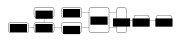
\includegraphics{./sdf/quantum_noise/figures/scheme_experimental.pdf}
	\caption{Experimental setup}
	\label{fig:experimental_homodyne_setup}
\end{figure}

%%%%%%%%%%%%%%%%%%%%%%%%%%%%%%%%%%%%%%%%%%%%%%%%%%%%%%%%%%%%%%%%%%%%%%%%%%%%%%%%
% References
%%%%%%%%%%%%%%%%%%%%%%%%%%%%%%%%%%%%%%%%%%%%%%%%%%%%%%%%%%%%%%%%%%%%%%%%%%%%%%%%

\renewcommand{\bibname}{References}
%
\bibliographystyle{myIEEEtran}
% argument is your BibTeX string definitions and bibliography database(s)
\bibliography{./sdf/quantum_noise/quantum_noise}
%
%


\cleardoublepage
